%!TEX root = ../template.tex
%%%%%%%%%%%%%%%%%%%%%%%%%%%%%%%%%%%%%%%%%%%%%%%%%%%%%%%%%%%%%%%%%%%
%% chapter1.tex
%% NOVA thesis document file
%%
%% Chapter with introduciton
%%%%%%%%%%%%%%%%%%%%%%%%%%%%%%%%%%%%%%%%%%%%%%%%%%%%%%%%%%%%%%%%%%%
\chapter{Experimental Observations and Validations}
\label{cha:experimentalEvaluation}

In this chapter we describe the work we conducted for the validation and evaluation of our proposed in-memory TREDIS solution. 

We start by presenting the metrics we intend to evaluate, along with the test benches we defined to test our prototype.
We then go deeper about each test bench, describing the results obtained during the experimental evaluation of each one of those scenarios, leading to a discussion later in this chapter aiming to compare those results and, finally, ending with a summary of the chapter.


\section{Criteria for Experimental Observations}
\label{sec:criteriaForExperimentalObservations}

Our evaluation process is simple: track our TREDIS solution's behavior through all the different configurations, incrementally adding more layers to the system. Thus, we intend to evaluate our TREDIS solution on each possible configuration, starting with a basic model and slowly add more components to the system, while also making experimental observations about the impact they have. 

During the evaluation process we focused on measuring: 1) the performance impact each component has in the system while running with or without \gls{sgx}, through latency and throughput analysis, and 2) resource allocation during runtime, including memory and CPU usage. 

There are other particular measurements that we found useful to introduce, that we detailed later, while describing the test benches individually.
Adding to that, we also analysed the system's behavior under different client-workloads, by scaling up the number of requests and varying the typology of requests made to the system.


\section{Deployment Of Testbench Environments}
\label{sec:testBenchEnvironments}

As said before, we intend to evaluate our in-memory TREDIS system behavior by incrementally adding components to it, which will add security to the whole system, and see what impact they have on it. In order to do that, we defined a list of Test Benches (TB) that helped us evaluate the system.

First, our idea was to benchmark the \gls{kvs} Redis layer running normally inside our cloud server, to use it as a reference point to what is the expected behavior of a in-memory Redis \gls{kvs} in our server, with the conditions we offered. Thus, we defined the TestBench 1 (TB1) as a default version of Redis, with TLS support.

As the next step, we analyzed the impact that \gls{sgx} has in a \gls{sgx}-enabled Redis. For that we defined TB2 as our server running the Redis \gls{kvs} component inside a SGX-enabled SCONE container.

TB3 includes the addition of the Proxy component, in order to benchmark its impact on the system. Thus, we defined TB3 as a Redis component running inside a SGX-enabled SCONE container, along with a Single Proxy instance.

In TB4, we placed the Proxy component on top of \gls{sgx}, resulting on benchmarking a system composed by the Redis \gls{kvs} running inside a SGX-enabled SCONE container, along with a Single Proxy instance also running inside \gls{sgx}.

For TB5, we added the attestation property to the components, used to assure that they run in private memory regions on top of \gls{sgx} and that they are only executed by the right enclave. Here we measure the impact it has to attestate each component upon start.

After that, with all the system model defined in \ref{cha:systemModel_and_design} in place, we created two more test benches TB6 and TB7 to evaluate the whole system behavior against different client request overloads (10k requests vs 100k requests and different size payloads) and against different typologies of requests (i.e., 10\% Writes:90\% Reads), respectively.

All these test benches were used to evaluate our soluution while running the Redis layer in all the three configurations we spoken in previous chapters: single instance Redis, Master-Slave Redis and Clustered Redis.


\section{Observations with Cloud-based Single REDIS}
\label{sec:cloudS_Redis}

In this section, we analize our solution running the in-memory Redis component configured as a single instance \gls{kvs}. The experimental evaluation will be done following the test benches defined above, in order to study the impact of \gls{sgx} in our system, analysing both the performance and resource allocation impact that each secured component has in the system.

As we detailed in \ref{sec:implementationArchitecture}, we run our solution on a cloud system with \gls{sgx}-enabled hardware, while our client benchmark applications run on a local machine with commodity hardware, in order to simulate a real-world use-case where the network has a major impact in the performance of a system.

\subsection{Latency Impact of SGX-Enabled REDIS}

To study and compare the latency levels of TREDIS with and without \gls{sgx}, we evaluated our solution by complying to the test benches TB1, TB2, TB3 and TB4 (see \ref{sec:testBenchEnvironments} for details) definitions, with network conditions of $\approx$116Mb/s Download and $\approx$114Mb/s Upload speed. It is important to mention that, for the first two test benches where our client applications point directly to the Redis \gls{kvs} layer, we used redis-benchmark to make the requests and benchmark the solution. However, with the addition of the Proxy layer in TB3, we had to switch to a HTTP-enabled client - Jmeter.

Thus, we started to benchmark our solution according to TB1, which resulted on an average 33,97 millisecond response time.
Comparing this value to the value of TB2, we observed that the addition of \gls{sgx} security properties to the \gls{kvs} component induced a latency penalty of 4,89\%, as we can see in Table \ref{table:latencySingleRedis}.

%\begin{figure}[htbp]
%	\centering
%	{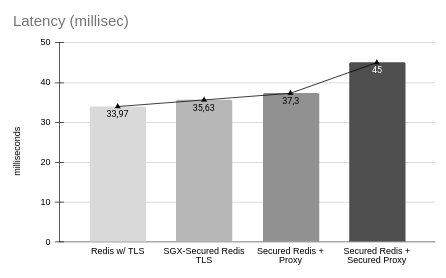
\includegraphics[width=0.8\linewidth]{graphLatency1234}}
%	\caption{Latency impact of SGX on single instance TREDIS}
%	\label{fig:graphLatencyStandalone}
%\end{figure}

\begin{table}[ht]
	\caption{Latency impact of SGX in Standalone Redis} % title of Table
	\centering % used for centering table
	\begin{tabular}{c c} % centered columns (4 columns)
		\hline\hline %inserts double horizontal lines
		\textbf{Configuration} & \textbf{Latency} \\ [0.5ex] % inserts table
		%heading
		\hline
		Redis & 33,97ms\\
		\hline
		SGX-enabled Redis & 35,63ms \\
		\hline
	    SGX-enabled Redis + Proxy & 37,3ms \\
		\hline % inserts single horizontal line
	    SGX-enabled Redis + SGX-enabled Proxy & 44ms\\ [1ex] % [1ex] adds vertical space
		\hline %inserts single line
	\end{tabular}
	\label{table:latencySingleRedis} % is used to refer this table in the text
\end{table}

However, as we detailed before in previous chapters, our TREDIS solution includes also a Proxy component that also adds overhead to the system, specially when also running inside \gls{sgx}. For that analysis, we run TB3 and TB4, in order to evaluate Proxy's impact in the overall system. Thus, with the addition of the Proxy, we observed an additional 4,69\% overhead compared to TB2, that we consider to be worth due to the purpose we give to this component. However, the 17,96\% latency increase that \gls{sgx} imposes to the Proxy component can lead to a subjective conclusion, depending on how important it is for the system to secure this entry point.

\subsection{Generic Throughput Observation}

In order to measure the impact that enabling \gls{sgx} has on the throughput of our solution, we followed the same test benches as the ones used in the latency test - TB1, TB2, TB3 and TB4. Our following evaluation is based on the average measurements of a few identical tests, each one consisting on one client (thread) making 10 000 requests with 10 Bytes worth of data over the network.

\begin{figure}[htbp]
	\centering
	{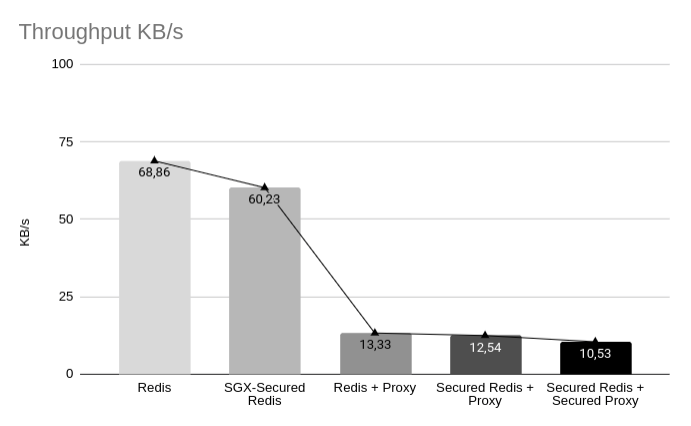
\includegraphics[width=0.8\linewidth]{graphThroughputStandalone}}
	\caption{SGX throughput impact - Standalone TREDIS}
	\label{fig:graphThroughputStandalone}
\end{figure}

Here, the addition of \gls{sgx} to the Redis component induced in a 12,53\% overhead, that can be observed in Figure \ref{fig:graphThroughputStandalone} in the tests made via redis-benchmark, in which the client application connects directly with the \gls{kvs} layer itself, via TCP. 

However, in TB3 and TB4, we can see that adding the Proxy component to the system dropped significantly the solution's throughput levels. This is expected since the requests started to be done via HTTP, which induces in losses of $\approx$80\% compared to TCP. With the requests being done to the Proxy, we observe only a 5,93\% throughput penalty on running the \gls{kvs} on top of \gls{sgx}, which can be seen in Table \ref{table:throughputSingleRedis}, along with a 16,02\% drop when enabling the Proxy layer to also execute on top of \gls{sgx}.


\begin{table}[ht]
	\caption{Throughput impact of SGX} % title of Table
	\centering % used for centering table
	\begin{tabular}{c c} % centered columns (4 columns)
		\hline\hline %inserts double horizontal lines
		\textbf{Configuration} & \textbf{Throughput} \\ [0.5ex] % inserts table
		%heading
		\hline
		Redis + Proxy & 13,33KB/s\\
		\hline
		SGX-enabled Redis + Proxy & 12,54KB/s \\
		\hline % inserts single horizontal line
		SGX-enabled Redis + SGX-enabled Proxy & 10,53KB/s\\ [1ex] % [1ex] adds vertical space
		\hline %inserts single line
	\end{tabular}
	\label{table:throughputSingleRedis} % is used to refer this table in the text
\end{table}

\begin{table}[ht]
	\caption{Attestation impact in boot time} % title of Table
	\centering % used for centering table
	\begin{tabular}{c c c} % centered columns (4 columns)
		\hline\hline %inserts double horizontal lines
		\textbf{} & \textbf{No Attestation} & \textbf{Attestation} \\ [0.5ex] % inserts table
		%heading
		\hline
		\textbf{Redis} & 0,14s & 1,37s\\
		\hline % inserts single horizontal line
		\textbf{Proxy} & 62,07s & 63,12\\ [1ex] % [1ex] adds vertical space
		\hline %inserts single line
	\end{tabular}
	\label{table:attestationImpactBoot} % is used to refer this table in the text
\end{table}

Total differences: Redis - 1,23s Proxy - 1,05s

(TODO TODO TODO) - Attestation

\subsection{Evaluation of Specific Benchmarks and Operations}
\label{ssec:specificBenchmarksRedisS}

As a way to evaluate our solution's behavior facing more specific benchmarks, we tested the service by following the TB6 and TB7. 

Here we present how different operation ratios influence the system throughput. By looking at Figure \ref{fig:thptDiffCombinationsSingleRedis}, we can see that there is not a big difference on how TREDIS handles these different combinations of requests with small payloads, which remain relatively stable, only showing a slight throughput advantage when the test consists in a majority of writes, in comparison to the tests a higher number of reads. This absence of difference might be related to the fact that Redis is able to handle a lot of requests per second, thus with small payloads, where it takes almost no time to compute, the numbers should look alike as they do.  

\begin{figure}[htbp]
	\centering
	{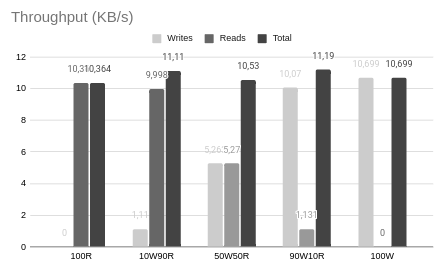
\includegraphics[width=0.8\linewidth]{thptDiffCombinationsSingleRedis}}
	\caption{SGX throughput impact - Standalone TREDIS}
	\label{fig:thptDiffCombinationsSingleRedis}
\end{figure}

However, with the increase of payload size, we start to see the oposite behavior, as we can see in the Table \ref{table:throughputPayloads}. This is due to the Redis-server needing more time to write more data into the database. On the other hand, reads allow (TODO TODO TODO)

\begin{table}[ht]
	\caption{Throughput differences with different size payloads} % title of Table
	\centering % used for centering table
	\begin{tabular}{c c c} % centered columns (4 columns)
		\hline\hline %inserts double horizontal lines
		\textbf{Payload Size} & \textbf{Read} & \textbf{Write} \\ [0.5ex] % inserts table
		%heading
		\hline
		10B & 10,364KB/s & 10,699KB/s\\
		\hline
		10KB & 208,33KB/s & 9,43KB/s \\
		\hline % inserts single horizontal line
		100KB & 1507,23KB/s & 5,31KB/s\\ [1ex] % [1ex] adds vertical space
		\hline %inserts single line
	\end{tabular}
	\label{table:throughputPayloads} % is used to refer this table in the text
\end{table} 

Also, to comply with TB6, we scaled the number of requests made to the server, in order to see differences in the behavior of the system. However, we found it hard to simulate \gls{epc} memory page swapping with small payloads, as it takes a long time to reach near the \gls{epc} memory size, so we incremented the size of the requests to 500KB. By doing that, we encountered an unexpected problem: when reaching the maximum heap size defined for Redis upon start, the container crashed. We later found out that this problem is targeted in SCONE's website\footnote{https://sconedocs.github.io/faq/}, where it is explained this happens due to the SGX version (SGX v1) we are using not supporting dynamic allocation of memory, thus \textit{"enclaves must allocate all memory at startup since enclaves are fixed"}. This causes the memory usage of Redis to be higher than it needs to be, since to prevent it from crashing, we need to allocate memory upon start that we don't know we will need, which leads to larger startup times. However, SCONE also affirms that the next version of SGX (SGX v2) will support dynamic allocation, which tackles this problem. 

Thus, in order to test the EPC swap impact in the system, we increased the heap size to 2GB(TODO TODO TODO)


\subsection{REDIS Standalone System Resources}

Here we evaluate our solution's memory consumption and CPU usage during runtime. 
For the purpose of this test, our client application made requests to the Proxy during 180s with 1KB worth of data.  

In the graphs we present in Figure \ref{fig:MemoryConsumption_standalone}, we observe some changes in the system when running it on top of \gls{sgx} and outside of it. First of all, we notice that the dataset size increases faster if running without \gls{sgx} support, since the system is faster and its throughput levels are higher, resulting in more operations made over the dataset in the same period. We can also see that the Resident Set Size (RSS) in one case is dynamic, while in the other is static. This calls back to what we stated in the section before, where we mentioned that SGX v1 does not support dynamic allocation of memory, thus only relying on the heap size specified upon creation which remains static throughout execution. In Figure \ref{fig:SgxStandaloneMemory} we see just that, a static RSS value throughout the entire evaluation. Note that this RSS value defined the memory available for Redis to scale during its execution. Thus, running Redis inside SGX might induce into memory problems if using SGX v1, since either the system reaches the point where it is left with no memory available to run and stops, or it is created with huge amounts of memory, which might not be necessary, while inducing into big startup times since it needs to allocate more memory upfront.

\begin{figure}[htbp]
	\centering
	\subbottom[Memory consumption without SGX]{%
		\label{fig:noSgxStandaloneMemory}
		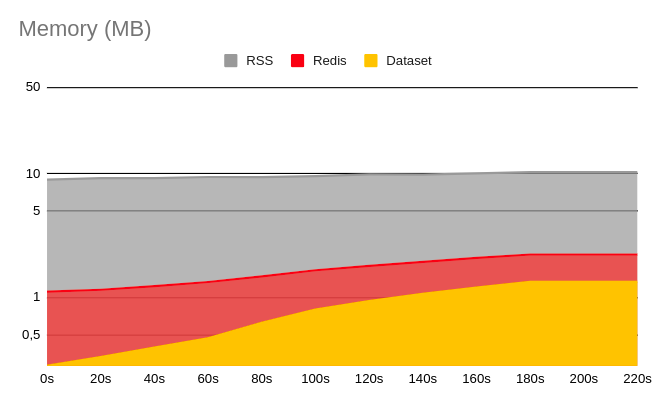
\includegraphics[width=0.5\linewidth]{memoryRedisNoSGX_standalone}}%
	\subbottom[Memory consumption with SGX]{
		\label{fig:SgxStandaloneMemory}
		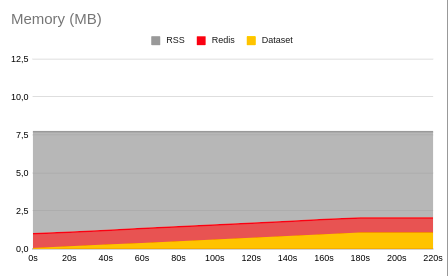
\includegraphics[width=0.5\linewidth]{memoryRedisSGX_standalone}}
	\caption{Redis Standalone memory consumption during runtime}
	\label{fig:MemoryConsumption_standalone}
\end{figure}

As for the CPU usage, we show in Figure \ref{fig:cpuUsageStandalone} the impact that \gls{sgx} has. On the left, we see the CPU resources that goes into the execution of the solution without this extra layer of security, remaining near 0\% for Redis while the Proxy shows values of around 5-8\%, due to being a Java application which includes a JVM and all its components running in the background alongside the Proxy. On the right, we see a more expressive set of results, where the addition of \gls{sgx} results on higher CPU usage, specially by the Proxy component. However, since this test induced in a high density of requests, we do not consider this results to be negative, nor unexpected.

\begin{figure}[htbp]
	\centering
	\subbottom[CPU usage without SGX]{%
		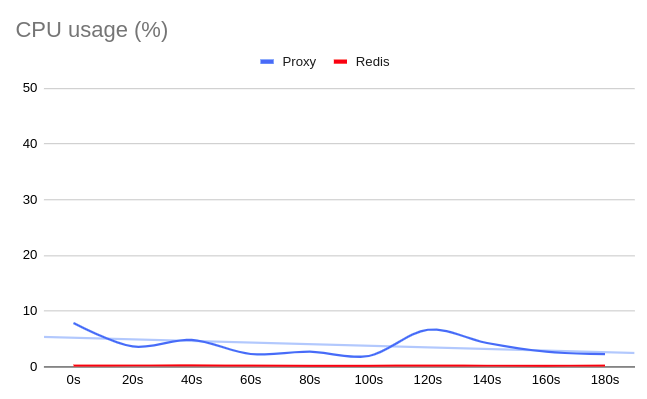
\includegraphics[width=0.5\linewidth]{cpuUsageStandalone_noSGX}}%
	\subbottom[CPU usage with SGX]{
		\label{fig:sgxCPUusage_standalone}
		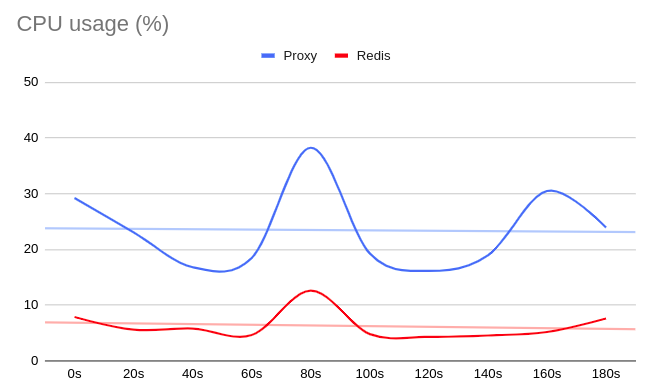
\includegraphics[width=0.5\linewidth]{cpuUsageStandalone}}
	\caption{Redis Standalone CPU usage during runtime}
	\label{fig:cpuUsageStandalone}
\end{figure}

\section{Observations with Cloud-based Master-Slave REDIS}
\label{sec:cloud_MS_Redis}

Here we present what we observed while testing our solution with the \gls{kvs} Redis layer in a Master-Slave configuration. We prepared it to run with three replicas, one being a Master node, and the other two being read-only Slave nodes. 

Hereupon, this experimental evaluation follows the same test benches that we used in Section \ref{sec:cloudS_Redis}, to analyze the impact that enabling \gls{sgx} support to our components have in the whole solution.

We run the test scenarios in the same environment previously used, in a cloud system with \gls{sgx} support, while making the requests in a local machine over the network. However, this time we registed  our network speed to be of $\approx$117Mb/s Download to $\approx$119Mb/s Upload.


\subsection{Latency and impact of SGX-Enabled Master-Slave REDIS}

In order to evaluate the latency impact of \gls{sgx} in our solution, as we just mentioned, we executed the TB1, TB2, TB3 and TB4 scenarios, incrementally adding components to the system, while enabling \gls{sgx} support to each one of them along the way. 

The test was similar, starting with redis-benchmark as the client application when communicating directly to the Redis-server, and Jmeter to communicate through HTTP with the Proxy component.

\begin{table}[ht]
	\caption{Latency impact of SGX in Standalone Redis} % title of Table
	\centering % used for centering table
	\begin{tabular}{c c} % centered columns (4 columns)
		\hline\hline %inserts double horizontal lines
		\textbf{Configuration} & \textbf{Latency} \\ [0.5ex] % inserts table
		%heading
		\hline
		Redis & 32,48ms\\
		\hline
		SGX-enabled Redis & 32,97ms \\
		\hline
		SGX-enabled Redis + Proxy & 34,45ms \\
		\hline % inserts single horizontal line
		SGX-enabled Redis + SGX-enabled Proxy & 41ms\\ [1ex] % [1ex] adds vertical space
		\hline %inserts single line
	\end{tabular}
	\label{table:latencyMasterSlaveRedis} % is used to refer this table in the text
\end{table}

In Table \ref{table:latencyMasterSlaveRedis} we can observe a similar behavior compared to the values we saw for our solution running a single instance Redis, as the latency time increases with the components and security we give to the system. Here we can see a 1,51\% drop with the addition of \gls{sgx} support to the \gls{kvs} layer. Connecting the Proxy costed the system around 4,49\%, while protecting it with \gls{sgx} induced the solution in a 19\% latency drop.

(TODO TODO TODO) try to explain why proxy loses so much latency

\subsection{Generic throughput comparative observations}
Our throughput evaluation was made with the same configuration used for Standalone Redis, consisting in one client thread doing all the 10 000 requests with a payload of 10 Bytes, while registering the average results of multiple tests.

In Figure \ref{fig:graphTroughputMasterSlave} we can observe a 7,15\% drop by securing the \gls{kvs} layer with \gls{sgx}, which is a slightly smaller loss than the one we observed in the Standalone tests. However, we observe once again a considerable penalty with the addition of the Proxy layer, which along with the switch from TCP requests to HTTP requests causes a huge throughtput drop of around 80\%, even without any \gls{sgx} inclusion. With the inclusion of this last one, our solution exhibits a loss of 15,45\%.

\begin{figure}[htbp]
	\centering
	{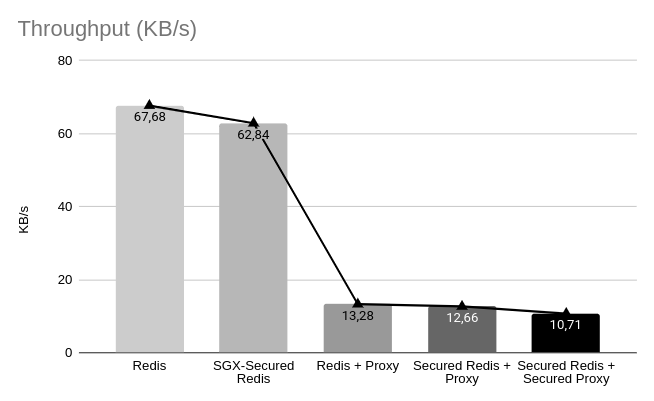
\includegraphics[width=0.8\linewidth]{graphThroughputMasterSlave}}
	\caption{SGX impact in MasterSlave}
	\label{fig:graphTroughputMasterSlave}
\end{figure}

(TODO TODO TODO) - Attestation

\subsection{Throughput with benchmarks and specific operations}

Here we tested the behavior of our Master-Slave configured solution against different operation ratios and different payload sizes. 
In Figure \ref{fig:thptDiffCombinationsMasterSlaveRedis} we can see pretty much the same results we had with Redis running in Standalone mode. However, in Table \ref{table:throughputPayloadsMS} we observe better results in Read operations for the Master-Slave configuration, as we increase the payload sizes. 

\begin{figure}[htbp]
	\centering
	{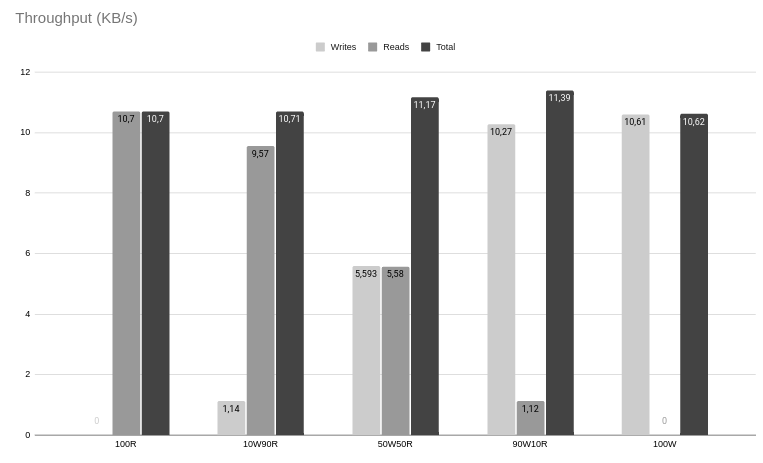
\includegraphics[width=0.8\linewidth]{thptDiffCombinationsMasterSlaveRedis}}
	\caption{SGX impact in MasterSlave}
	\label{fig:thptDiffCombinationsMasterSlaveRedis}
\end{figure}

\begin{table}[ht]
	\caption{Throughput differences with different size payloads} % title of Table
	\centering % used for centering table
	\begin{tabular}{c c c} % centered columns (4 columns)
		\hline\hline %inserts double horizontal lines
		\textbf{Payload Size} & \textbf{Read} & \textbf{Write} \\ [0.5ex] % inserts table
		%heading
		\hline
		10B & 10,7KB/s & 10,61KB/s\\
		\hline
		10KB & 230,75KB/s & 9,88KB/s \\
		\hline % inserts single horizontal line
		100KB & 1603,4KB/s & 4,76KB/s\\ [1ex] % [1ex] adds vertical space
		\hline %inserts single line
	\end{tabular}
	\label{table:throughputPayloadsMS} % is used to refer this table in the text
\end{table} 

This is justified due to read requests being now handled by all Redis replicas, since all are enable to execute reads. However, we see a slight drop in the write throughput values, since they are all handled by one replica, the Master-node, which has to also replicate the data to all replicas, after.


\subsection{M/S REDIS and Cloud system resources}


To evaluate, we tested the solution during 180s with requests of 1KB payload size.  



\begin{figure}[htbp]
	\centering
	\subbottom[CPU usage without SGX]{%
		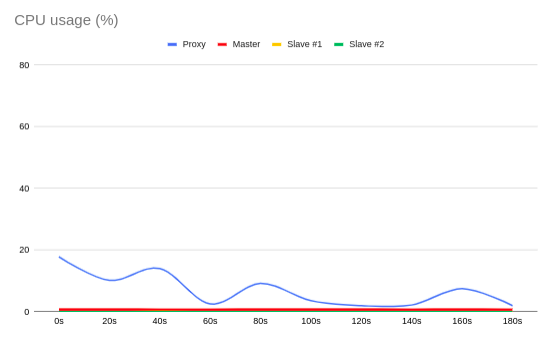
\includegraphics[width=0.51\linewidth]{cpuUsageMasterSlave_noSGX}}%
	\subbottom[CPU usage with SGX]{
		\label{fig:sgxCPUusage}
		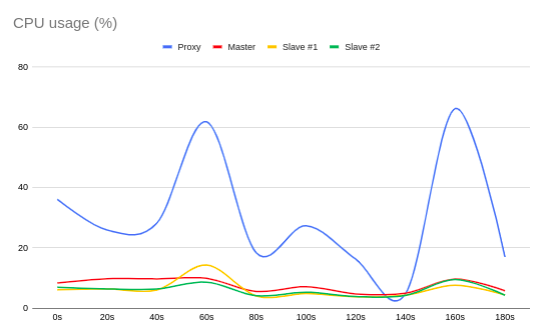
\includegraphics[width=0.51\linewidth]{cpuUsageMasterSlave}}
	\caption{Redis-SGX memory consumption during runtime}
	\label{fig:cpuUsage}
\end{figure}

the increase on CPU workload by the Redis instance is caused by the replication happening behind the scenes, between the master node and slaves.

SGX makes that RSS doesn't change, as we said in \ref{ssec:specificBenchmarksRedisS}, it's defined at boot and stays static throughout the execution. It shows the memory available for Redis to scale.
The other measurements, all normal.
The graphs are similar, where the slaves have the same memory usage (which makes sense since they store the same data), while the master occupies slightly more memory, probably due to replication delays, which end up to stable at the end.
As for Proxy memory usage, we were only able to obtain the 59MB from it's heap size defined by default for Java applications



\begin{figure}[htbp]
	\centering
	\subbottom[Master-node Memory consumption]{%
		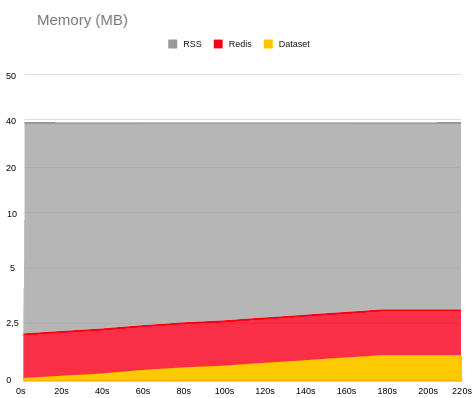
\includegraphics[width=0.5\linewidth]{memoryRedisSGXMS}}%
	\subbottom[Slave-node Memory consumption]{
		\label{fig:sgxSlaveMemory}
		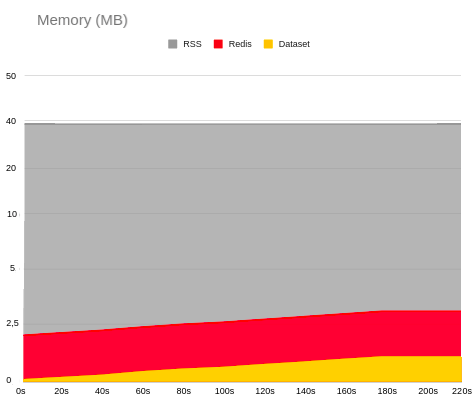
\includegraphics[width=0.5\linewidth]{memoryRedisSGXMS_slave}}
	\caption{Redis-SGX memory consumption during runtime}
	\label{fig:sgxMemoryConsumption}
\end{figure}

\begin{figure}[htbp]
	\centering
	\subbottom[Master-node Memory consumption]{%
		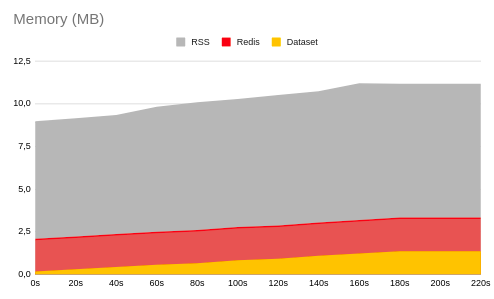
\includegraphics[width=0.5\linewidth]{memoryRedisNoSGX}}%
	\subbottom[Slave-node Memory consumption]{
		\label{fig:noSgxSlaveMemory}
		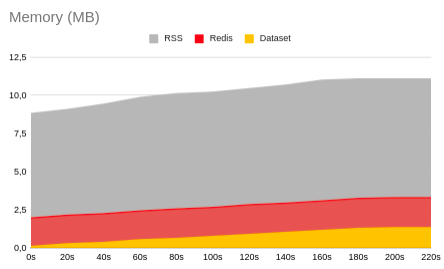
\includegraphics[width=0.5\linewidth]{memoryRedisNoSGX_slave}}
	\caption{Redis memory consumption during runtime}
	\label{fig:noSgxMemoryConsumption}
\end{figure}

\section{Observations with Cloud-based Clustered REDIS}
Mm cena mas po cluster

\subsection{Latency and impact of SGX-enabled REDIS Cluster}

\subsection{Comparative throughput: S  vs. M/S vs. CLUSTERED Redis}

\subsection{Clustered REDIS and Cloud System resources}

\section{Main findings from the experimental observations}

Comparar o 5.3, 5.4 e 5.5

Why proxy with all those losses? because we can expose an API to many regular users, and is a more real-world example of the possible use of a system like this + all the access control and entry point bullshit

\section{Summary}


